\documentclass{article}\usepackage[]{graphicx}\usepackage[]{color}
%% maxwidth is the original width if it is less than linewidth
%% otherwise use linewidth (to make sure the graphics do not exceed the margin)
\makeatletter
\def\maxwidth{ %
  \ifdim\Gin@nat@width>\linewidth
    \linewidth
  \else
    \Gin@nat@width
  \fi
}
\makeatother

\definecolor{fgcolor}{rgb}{0.345, 0.345, 0.345}
\newcommand{\hlnum}[1]{\textcolor[rgb]{0.686,0.059,0.569}{#1}}%
\newcommand{\hlstr}[1]{\textcolor[rgb]{0.192,0.494,0.8}{#1}}%
\newcommand{\hlcom}[1]{\textcolor[rgb]{0.678,0.584,0.686}{\textit{#1}}}%
\newcommand{\hlopt}[1]{\textcolor[rgb]{0,0,0}{#1}}%
\newcommand{\hlstd}[1]{\textcolor[rgb]{0.345,0.345,0.345}{#1}}%
\newcommand{\hlkwa}[1]{\textcolor[rgb]{0.161,0.373,0.58}{\textbf{#1}}}%
\newcommand{\hlkwb}[1]{\textcolor[rgb]{0.69,0.353,0.396}{#1}}%
\newcommand{\hlkwc}[1]{\textcolor[rgb]{0.333,0.667,0.333}{#1}}%
\newcommand{\hlkwd}[1]{\textcolor[rgb]{0.737,0.353,0.396}{\textbf{#1}}}%

\usepackage{framed}
\makeatletter
\newenvironment{kframe}{%
 \def\at@end@of@kframe{}%
 \ifinner\ifhmode%
  \def\at@end@of@kframe{\end{minipage}}%
  \begin{minipage}{\columnwidth}%
 \fi\fi%
 \def\FrameCommand##1{\hskip\@totalleftmargin \hskip-\fboxsep
 \colorbox{shadecolor}{##1}\hskip-\fboxsep
     % There is no \\@totalrightmargin, so:
     \hskip-\linewidth \hskip-\@totalleftmargin \hskip\columnwidth}%
 \MakeFramed {\advance\hsize-\width
   \@totalleftmargin\z@ \linewidth\hsize
   \@setminipage}}%
 {\par\unskip\endMakeFramed%
 \at@end@of@kframe}
\makeatother

\definecolor{shadecolor}{rgb}{.97, .97, .97}
\definecolor{messagecolor}{rgb}{0, 0, 0}
\definecolor{warningcolor}{rgb}{1, 0, 1}
\definecolor{errorcolor}{rgb}{1, 0, 0}
\newenvironment{knitrout}{}{} % an empty environment to be redefined in TeX

\usepackage{alltt}
\IfFileExists{upquote.sty}{\usepackage{upquote}}{}
\begin{document}

\begin{knitrout}
\definecolor{shadecolor}{rgb}{0.969, 0.969, 0.969}\color{fgcolor}\begin{kframe}
\begin{alltt}
\hlcom{#GUIA 16}

\hlcom{# tm= tama�o de la muestra}
\hlstd{tm}\hlkwb{=}\hlnum{100}\hlstd{; n} \hlkwb{<-} \hlnum{10}\hlstd{; p} \hlkwb{<-} \hlnum{0.25}
\hlcom{#generando las 100 n�meros aleatorios}
\hlstd{S} \hlkwb{=} \hlkwd{rbinom}\hlstd{(tm, n, p)}
\hlcom{# estandarizando cada una de las observaciones}
\hlstd{Z} \hlkwb{=} \hlstd{(S}\hlopt{-}\hlstd{n}\hlopt{*}\hlstd{p)}\hlopt{/}\hlkwd{sqrt}\hlstd{(n}\hlopt{*}\hlstd{p}\hlopt{*}\hlstd{(}\hlnum{1}\hlopt{-}\hlstd{p)); Z}
\end{alltt}
\begin{verbatim}
##   [1] -1.0954451 -0.3651484  1.8257419 -0.3651484 -0.3651484 -0.3651484
##   [7]  1.8257419 -1.8257419 -1.0954451  1.8257419  0.3651484  1.0954451
##  [13] -0.3651484 -0.3651484 -0.3651484  0.3651484  0.3651484  0.3651484
##  [19] -1.0954451 -1.0954451 -1.8257419  0.3651484  0.3651484 -1.0954451
##  [25] -1.0954451 -0.3651484  0.3651484  1.0954451 -0.3651484  0.3651484
##  [31]  0.3651484  1.8257419 -0.3651484 -0.3651484  0.3651484 -0.3651484
##  [37] -0.3651484  0.3651484  1.0954451  0.3651484 -0.3651484 -1.0954451
##  [43]  0.3651484 -0.3651484  1.0954451 -0.3651484  0.3651484 -1.8257419
##  [49] -1.0954451  1.0954451 -1.0954451  0.3651484  1.8257419 -1.8257419
##  [55]  1.0954451  0.3651484 -1.0954451  0.3651484 -0.3651484 -1.0954451
##  [61] -0.3651484 -1.0954451  1.8257419 -1.8257419  1.0954451 -1.0954451
##  [67] -0.3651484  1.0954451 -0.3651484 -1.0954451 -0.3651484  0.3651484
##  [73]  0.3651484 -1.0954451 -1.0954451  1.0954451 -1.8257419  1.0954451
##  [79]  0.3651484  0.3651484 -1.0954451  0.3651484  1.8257419 -1.0954451
##  [85] -1.0954451  0.3651484 -1.0954451 -1.0954451 -0.3651484  0.3651484
##  [91] -1.0954451 -1.0954451 -1.0954451 -0.3651484  0.3651484  0.3651484
##  [97] -0.3651484  1.0954451  1.8257419 -0.3651484
\end{verbatim}
\begin{alltt}
\hlkwd{hist}\hlstd{(Z,} \hlkwc{main}\hlstd{=}\hlstr{"Histograma de Z ~ N(0, 1)"}\hlstd{,} \hlkwc{xlab}\hlstd{=}\hlstr{"z = n�mero binomiales est�ndarizados"}\hlstd{,}
\hlkwc{ylab}\hlstd{=}\hlstr{"f(z)"}\hlstd{,} \hlkwc{prob}\hlstd{=}\hlnum{TRUE}\hlstd{,} \hlkwc{col}\hlstd{=}\hlstr{"khaki"}\hlstd{)}
\hlkwd{curve}\hlstd{(}\hlkwd{dnorm}\hlstd{(x,} \hlnum{0}\hlstd{,} \hlnum{1}\hlstd{),} \hlkwc{col} \hlstd{=} \hlstr{"deepskyblue"}\hlstd{,} \hlkwc{lty}\hlstd{=}\hlnum{2}\hlstd{,} \hlkwc{lwd}\hlstd{=}\hlnum{2}\hlstd{,} \hlkwc{add}\hlstd{=}\hlnum{TRUE}\hlstd{)}
\end{alltt}
\end{kframe}
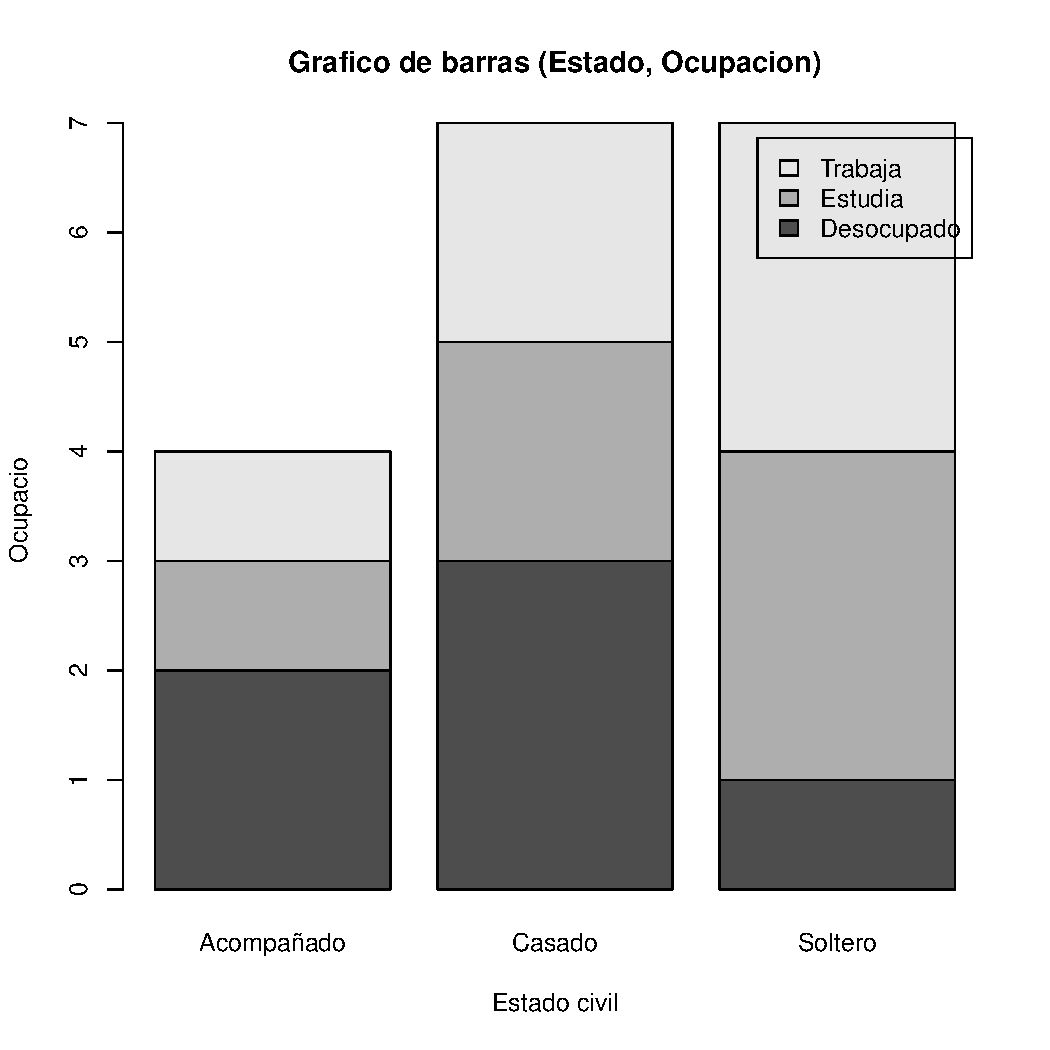
\includegraphics[width=\maxwidth]{figure/unnamed-chunk-1-1} 
\begin{kframe}\begin{alltt}
\hlstd{simulNorm} \hlkwb{<-} \hlkwa{function}\hlstd{(}\hlkwc{mu}\hlstd{,} \hlkwc{sigma}\hlstd{,} \hlkwc{m}\hlstd{=}\hlnum{5}\hlstd{,} \hlkwc{n}\hlstd{=}\hlnum{100}\hlstd{)}
\hlstd{\{}
\hlstd{vectMedias} \hlkwb{<<-} \hlkwd{numeric}\hlstd{(}\hlnum{0}\hlstd{)}
\hlstd{MediasEstand} \hlkwb{<<-} \hlkwd{numeric}\hlstd{(}\hlnum{0}\hlstd{)}
\hlkwa{for} \hlstd{(i} \hlkwa{in} \hlnum{1}\hlopt{:}\hlstd{m)}
\hlstd{\{}
\hlstd{X} \hlkwb{=} \hlkwd{rnorm}\hlstd{(n, mu, sigma)}
\hlcom{# genera n valores normales}
\hlstd{vectMedias[i]} \hlkwb{<<-} \hlkwd{mean}\hlstd{(X)}
\hlstd{MediasEstand[i]} \hlkwb{<<-} \hlstd{(vectMedias[i]} \hlopt{-} \hlstd{mu)}\hlopt{/}\hlstd{(sigma}\hlopt{/}\hlkwd{sqrt}\hlstd{(n))}
\hlstd{\}}
\hlstd{\}}
\hlstd{mu}\hlkwb{=}\hlnum{5}\hlstd{; sigma}\hlkwb{=}\hlnum{5}
\hlstd{m} \hlkwb{<-} \hlnum{200}
\hlcom{# n�mero de muestras o medias a obtener}
\hlkwd{simulNorm}\hlstd{(mu, sigma, m)}
\hlkwd{hist}\hlstd{(MediasEstand,} \hlkwc{main}\hlstd{=}\hlstr{"Histograma de medias est�ndarizadas"}\hlstd{,} \hlkwc{xlab}\hlstd{=}\hlstr{"Valores de m
medias normales est�ndarizadas"}\hlstd{,} \hlkwc{prob}\hlstd{=}\hlnum{TRUE}\hlstd{,} \hlkwc{col}\hlstd{=}\hlstr{"darkolivegreen3"}\hlstd{)}
\hlkwd{curve}\hlstd{(}\hlkwd{dnorm}\hlstd{(x,} \hlnum{0}\hlstd{,} \hlnum{1}\hlstd{),} \hlkwc{col} \hlstd{=} \hlstr{"deeppink3"}\hlstd{,} \hlkwc{lty}\hlstd{=}\hlnum{2}\hlstd{,} \hlkwc{lwd}\hlstd{=}\hlnum{2}\hlstd{,} \hlkwc{add}\hlstd{=}\hlnum{TRUE}\hlstd{)}
\end{alltt}
\end{kframe}
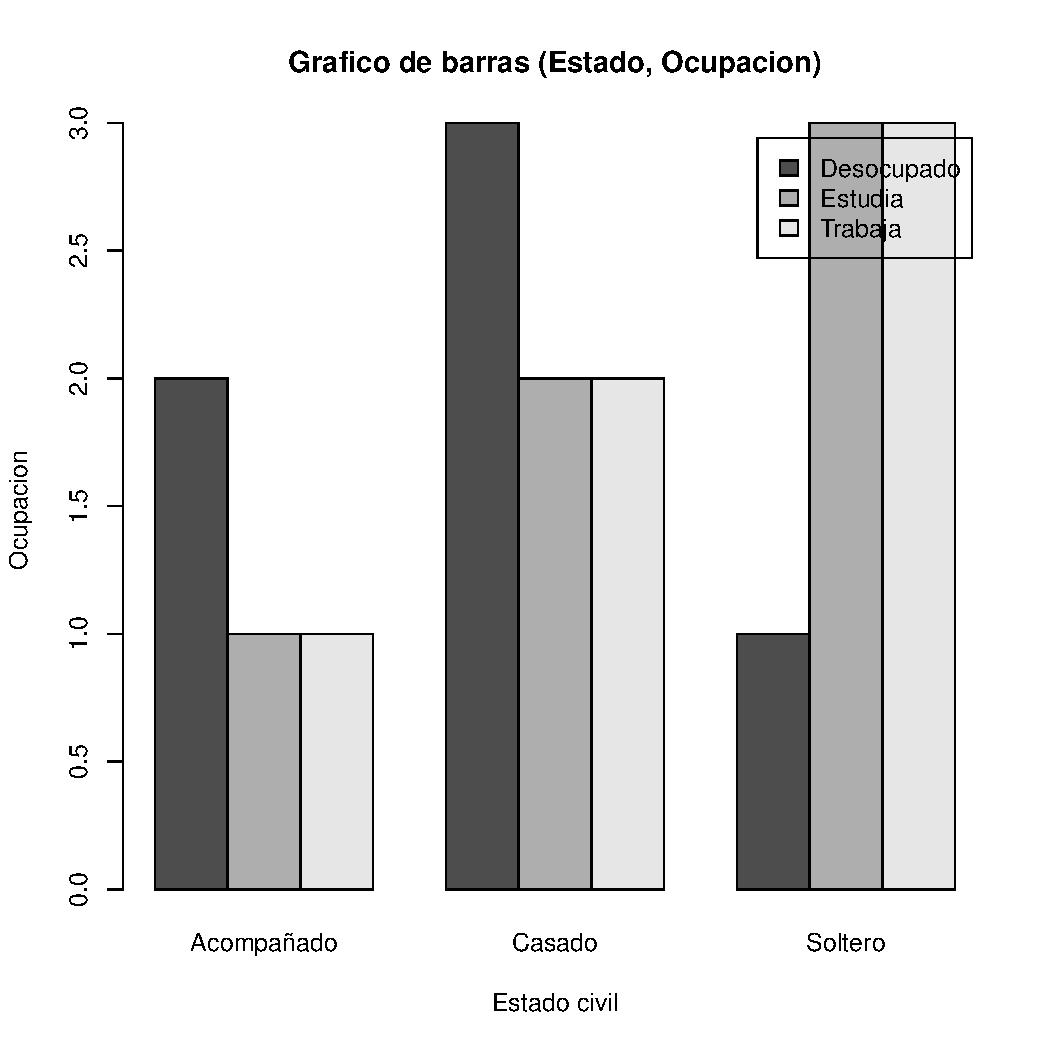
\includegraphics[width=\maxwidth]{figure/unnamed-chunk-1-2} 
\begin{kframe}\begin{alltt}
\hlkwd{qqnorm}\hlstd{(MediasEstand,} \hlkwc{main}\hlstd{=}\hlstr{"X ~ N(0, 1)"}\hlstd{)}
\hlcom{#muestra la l�nea}
\hlkwd{qqline}\hlstd{(MediasEstand,} \hlkwc{lty}\hlstd{=}\hlnum{1}\hlstd{,} \hlkwc{lwd}\hlstd{=}\hlnum{2}\hlstd{,} \hlkwc{col}\hlstd{=}\hlstr{"red"}\hlstd{)}
\end{alltt}
\end{kframe}
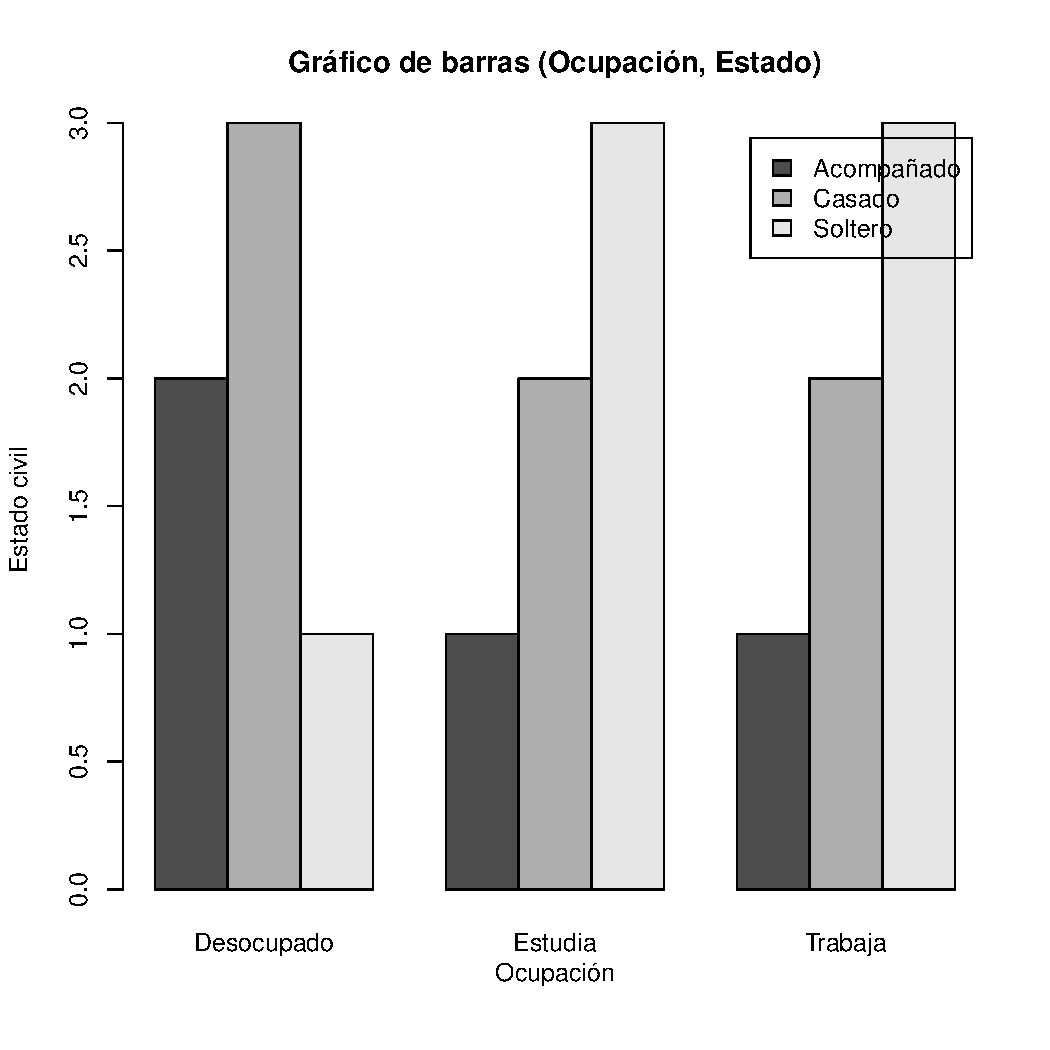
\includegraphics[width=\maxwidth]{figure/unnamed-chunk-1-3} 
\begin{kframe}\begin{alltt}
\hlstd{simulExp} \hlkwb{<-} \hlkwa{function}\hlstd{(}\hlkwc{mu}\hlstd{,} \hlkwc{m}\hlstd{=}\hlnum{5}\hlstd{,} \hlkwc{n}\hlstd{=}\hlnum{100}\hlstd{)}
\hlstd{\{}
\hlstd{razon} \hlkwb{<-} \hlnum{1}\hlopt{/}\hlstd{mu}
\hlstd{vectMedias} \hlkwb{<<-} \hlkwd{numeric}\hlstd{(}\hlnum{0}\hlstd{)}
\hlstd{MediasEstand} \hlkwb{<<-} \hlkwd{numeric}\hlstd{(}\hlnum{0}\hlstd{)}
\hlkwa{for} \hlstd{(i} \hlkwa{in} \hlnum{1}\hlopt{:}\hlstd{m)}
\hlstd{\{}
\hlstd{X} \hlkwb{=} \hlkwd{rexp}\hlstd{(n, razon)}
\hlcom{# genera n valores exponenciales}
\hlstd{vectMedias[i]} \hlkwb{<<-} \hlkwd{mean}\hlstd{(X)}
\hlstd{MediasEstand[i]} \hlkwb{<<-} \hlstd{(vectMedias[i]} \hlopt{-} \hlstd{mu)}\hlopt{/}\hlstd{(mu}\hlopt{/}\hlkwd{sqrt}\hlstd{(n))}
\hlstd{\}}
\hlstd{\}}
\hlkwd{par}\hlstd{(}\hlkwc{mfrow}\hlstd{=}\hlkwd{c}\hlstd{(}\hlnum{2}\hlstd{,}\hlnum{2}\hlstd{))}
\hlcom{# para n=1}
\hlstd{mu}\hlkwb{=}\hlnum{10}
\hlstd{m} \hlkwb{<-} \hlnum{100}\hlstd{; n} \hlkwb{<-} \hlnum{1}
\hlkwd{simulExp}\hlstd{(mu, m, n)}
\hlkwd{hist}\hlstd{(MediasEstand,} \hlkwc{main}\hlstd{=}\hlstr{"Medias Exp(10); n=1"}\hlstd{,} \hlkwc{xlab}\hlstd{=}\hlstr{"m medias exp est�ndarizadas"}\hlstd{,}
\hlkwc{prob}\hlstd{=}\hlnum{TRUE}\hlstd{,} \hlkwc{col}\hlstd{=}\hlstr{"darkolivegreen3"}\hlstd{)}
\hlstd{xvals} \hlkwb{=} \hlkwd{seq}\hlstd{(}\hlkwc{from}\hlstd{=}\hlopt{-}\hlnum{3}\hlstd{,} \hlkwc{to}\hlstd{=}\hlnum{3}\hlstd{,} \hlkwc{by}\hlstd{=}\hlnum{0.01}\hlstd{)}
\hlkwd{points}\hlstd{(xvals,} \hlkwd{dnorm}\hlstd{(xvals,} \hlnum{0}\hlstd{,} \hlnum{1}\hlstd{),} \hlkwc{col} \hlstd{=} \hlstr{"red"}\hlstd{,} \hlkwc{type}\hlstd{=}\hlstr{"l"}\hlstd{,} \hlkwc{lty}\hlstd{=}\hlnum{1}\hlstd{,} \hlkwc{lwd}\hlstd{=}\hlnum{2}\hlstd{)}

\hlcom{# para n=5}
\hlstd{n} \hlkwb{<-} \hlnum{5}
\hlkwd{simulExp}\hlstd{(mu, m, n)}
\hlkwd{hist}\hlstd{(MediasEstand,} \hlkwc{main}\hlstd{=}\hlstr{"Medias Exp(10); n=5"}\hlstd{,} \hlkwc{xlab}\hlstd{=}\hlstr{"m medias exp est�ndarizadas"}\hlstd{,}
\hlkwc{prob}\hlstd{=}\hlnum{TRUE}\hlstd{,} \hlkwc{col}\hlstd{=}\hlstr{"darkolivegreen3"}\hlstd{)}
\hlstd{xvals} \hlkwb{=} \hlkwd{seq}\hlstd{(}\hlkwc{from}\hlstd{=}\hlopt{-}\hlnum{3}\hlstd{,} \hlkwc{to}\hlstd{=}\hlnum{3}\hlstd{,} \hlkwc{by}\hlstd{=}\hlnum{0.01}\hlstd{)}
\hlkwd{points}\hlstd{(xvals,} \hlkwd{dnorm}\hlstd{(xvals,} \hlnum{0}\hlstd{,} \hlnum{1}\hlstd{),} \hlkwc{col} \hlstd{=} \hlstr{"red"}\hlstd{,} \hlkwc{type}\hlstd{=}\hlstr{"l"}\hlstd{,} \hlkwc{lty}\hlstd{=}\hlnum{1}\hlstd{,} \hlkwc{lwd}\hlstd{=}\hlnum{2}\hlstd{)}
\end{alltt}
\end{kframe}
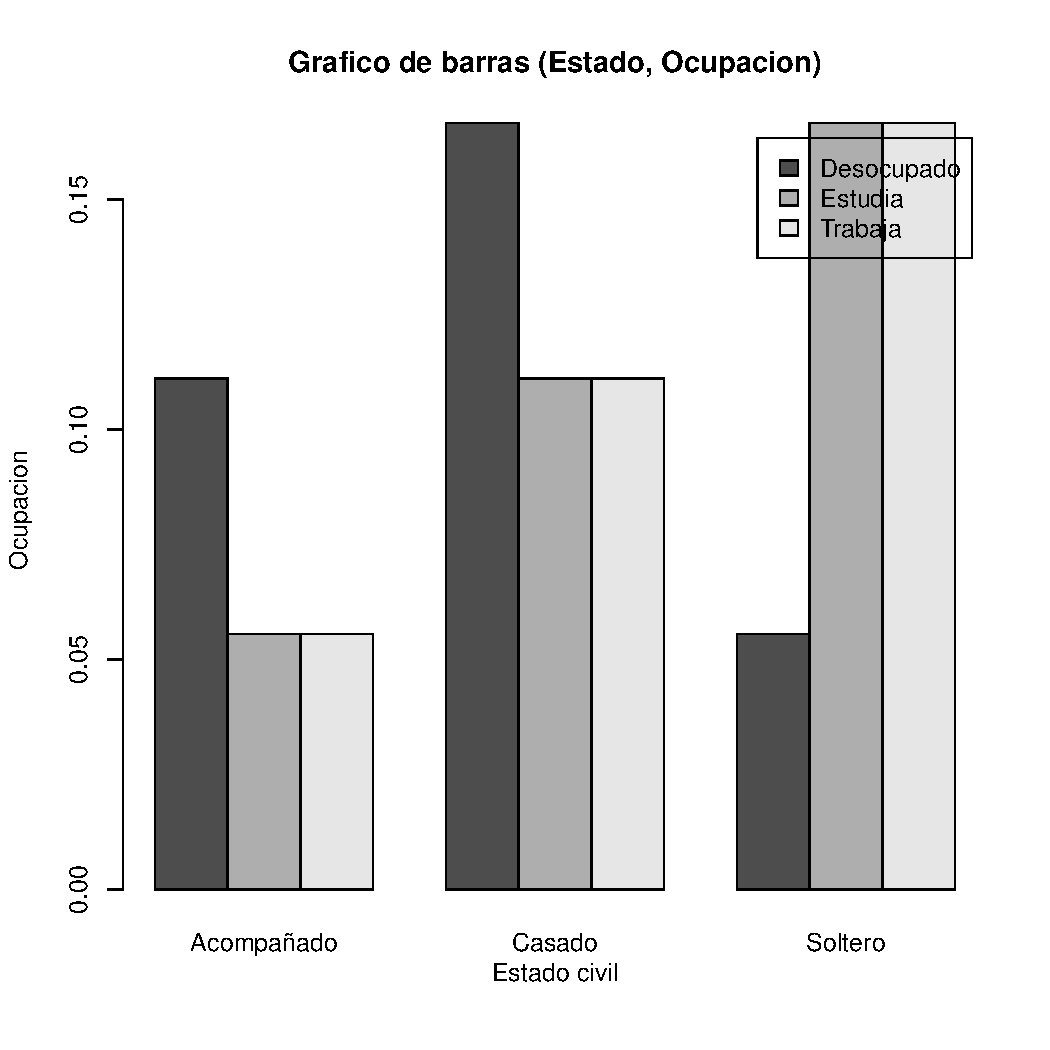
\includegraphics[width=\maxwidth]{figure/unnamed-chunk-1-4} 

\end{knitrout}



\end{document}
